\section{Numerical test cases}
\label{sec:num_cases}
In this section we present solutions to the linear advection equation using the C1FR scheme to show that it is stable and achieves the theoretical order of convergence of $P+1$ when the solution is discretized with an order $P$ polynomial. In addition, we present solutions to the linear advection-diffusion equation to demonstrate the ability to change the scheme's dispersion and dissipation properties while maintaining stability.

As can be seen from the derivation of the \gls{c1fr} scheme, the interface flux constants $\alpha_0$ and $\alpha_1$, the norm constants $c_0$ and $c_1$, and the location of the solution points at each element are variable. In this exposition, we will not modify the location of the solution points and use the standard zeroes of the Legendre polynomials. We note that the values of $c_1$ have a direct impact on the scheme's dispersion and dissipation, while --as expected-- the $\alpha_r$ values affect the dissipation only. A future rigorous Fourier analysis would reveal wiser choices for the $c_1$ parameter.


\subsection{Order of Accuracy of C1FR}
\subsubsection{Setup}

The 1-D experiments follow the procedure suggested by Vincent et al.~\cite{vincent2011insights} to estimate  a scheme's order of accuracy isolating interpolation errors. We solve the linear advection equation with advection speed of $a = 1$. The domain was $\Omega = [-10, 10]$ and was discretized in $n = 10, 15, 24, 38, 60$ equispaced elements of orders $P = 1,2,3$. The initial condition was a sine wave with wavenumber $k = 2\pi/20 \approx 0.63$. The advection speed was $1$ and fully upwinded fluxes $\alpha_0 = 0, \alpha_1 = 0$ in Eqn. \eqref{eq:ifluxdef}) were used. The boundary conditions were periodic. The simulation advanced using a fourth order \gls{rk} scheme with a time-step of order $10^{-3}$.

The initial condition was advected for a full domain length, using either standard nodal DG or \gls{c1fr}, and the resulting solution was taken as the reference solution $u_{ref}$. The wave was advected for a further full domain length to obtain the final solution $u_{final}$. The error was calculated by taking the L-2 norm of $u_{ref} - u_{final}$.

\subsubsection{Results and discussion}
Figures \ref{fig:adv_P1},\ref{fig:adv_P2}, and \ref{fig:adv_P3} show the rate of convergence of the solution and its derivative obtained by discretizing the solution wih polynomials of order $P = 1,2,3$, respectively. The slopes of the best fit lines are presented in each figure's caption.

\begin{figure}[h]
\centering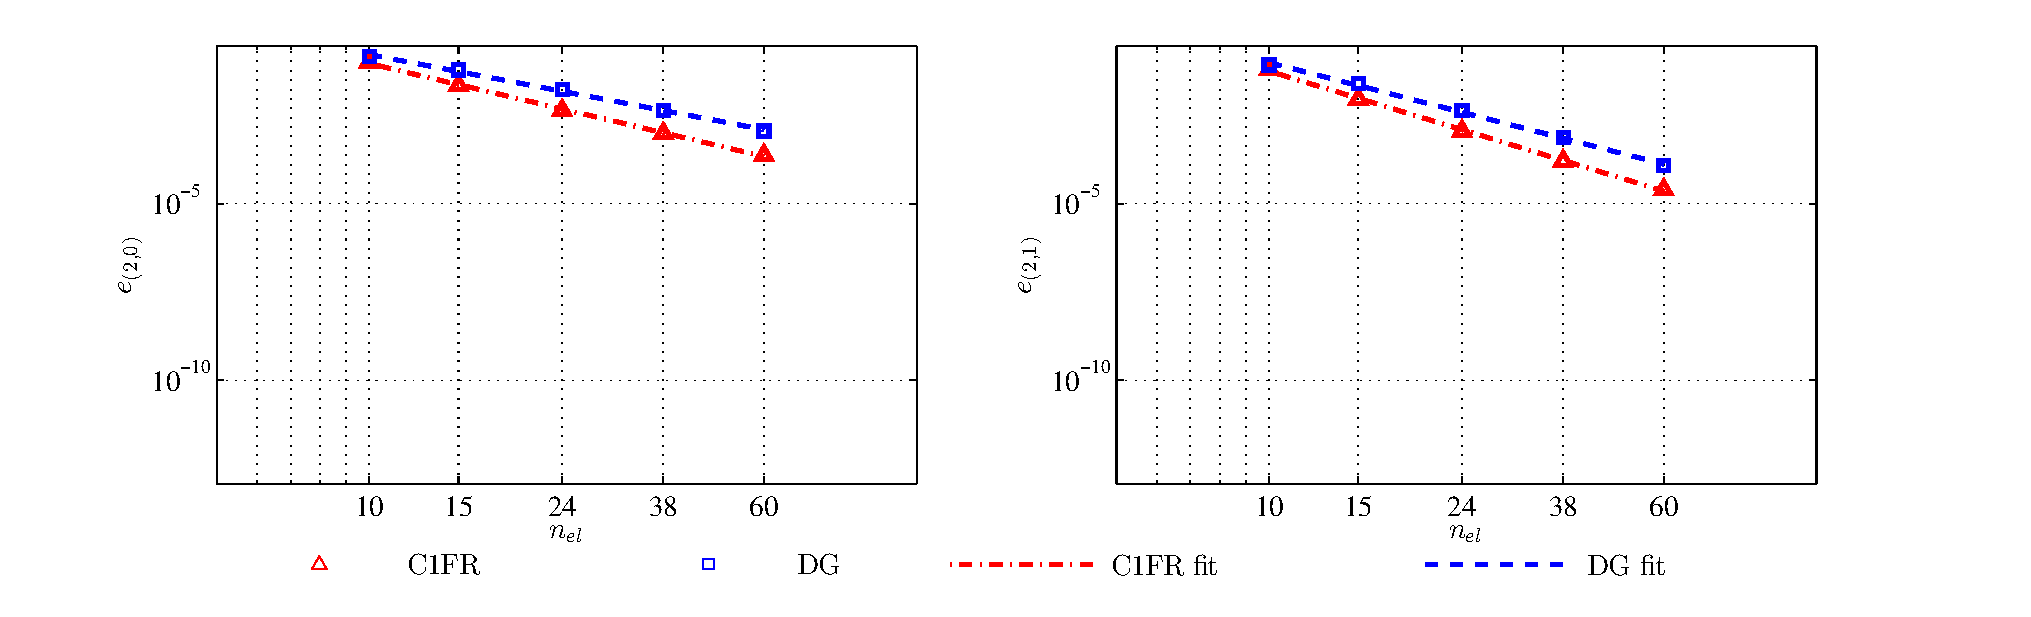
\includegraphics[width=1\textwidth,trim=\Ltrim cm 0cm \Rtrim cm 0cm]{\cmfrdir/Figures/Order_accuracy/P_1}
\caption{L-2 norm of error of advected sine wave and its derivative, $e_{(2,0)}$ and $e_{(2,1)}$ respectively, versus number of elements, for linear advection with polynomial discretization of order $P = 1$. Order of accuracy in solution: \gls{dg}: $2.728$, \gls{c1fr}: $3.374$. Order of accuracy in first derivative: \gls{dg}: $2.691$, \gls{c1fr}: $3.359$.}
\label{fig:adv_P1}
\end{figure}

\begin{figure}[h]
\centering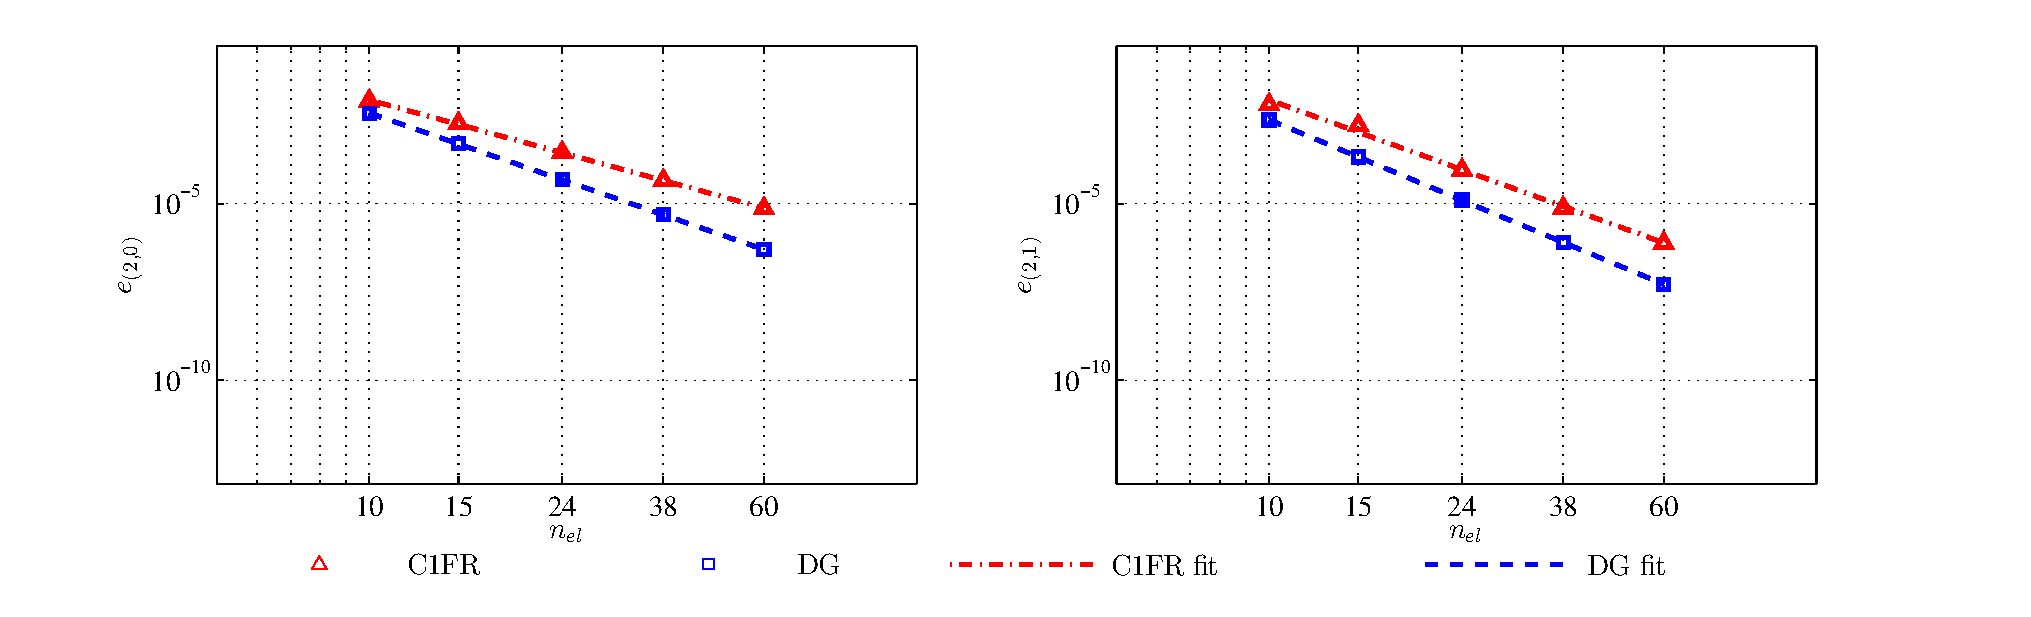
\includegraphics[width=1\textwidth,trim=\Ltrim cm 0cm \Rtrim cm 0cm]{\cmfrdir/Figures/Order_accuracy/P_2}
\caption{L-2 norm of error of advected sine wave and its derivative, $e_{(2,0)}$ and $e_{(2,1)}$ respectively, versus number of elements, for linear advection with polynomial discretization of order $P = 2$. Order of accuracy in solution: \gls{dg}: $4.960$, \gls{c1fr}:  $3.917$ . Order of accuracy in first derivative: \gls{dg}: $4.971$, \gls{c1fr}: $4.178$.}
\label{fig:adv_P2}
\end{figure}

\begin{figure}[h]
\centering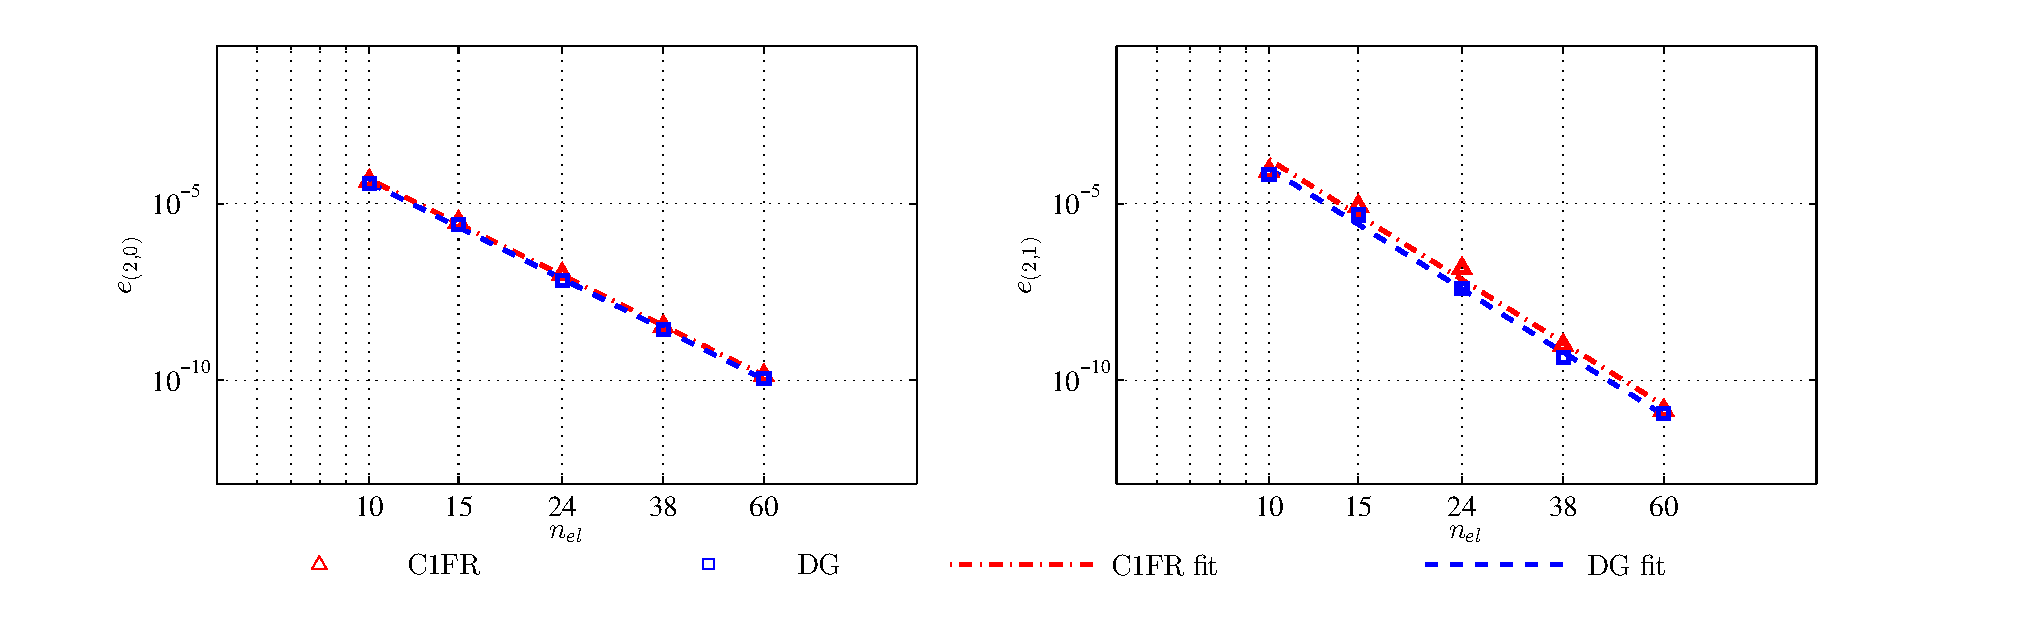
\includegraphics[width=1\textwidth,trim=\Ltrim cm 0cm \Rtrim cm 0cm]{\cmfrdir/Figures/Order_accuracy/P_3}
\caption{L-2 norm of error of advected sine wave and its derivative, $e_{(2,0)}$ and $e_{(2,1)}$ respectively, versus number of elements, for linear advection with polynomial discretization of order $P = 3$. Order of accuracy in solution: \gls{dg}: 7.119, \gls{c1fr}: 7.187. Order of accuracy in first derivative: \gls{dg}: 7.908, \gls{c1fr}: 7.882.}
\label{fig:adv_P3}
\end{figure}

The fact that we recover the expected nodal \gls{dg}'s $2P+1$ order of convergence found by Vincent et al. \cite{vincent2011insights} for $P = 1,2,3$ validates the experimental setup. It is interesting to note that \gls{c1fr} retains \gls{fr}'s even-odd order of convergence behavior: when $P$ is odd, the order of convergence is $2P+1$; while when $P$ is even, the order of convergence is $2P$.

This numerical experiment does not replace a von Neumann analysis, but does show that the scheme is stable, consistent, and maintains the desired order of accuracy. Although we would not expect the scheme to maintain super-convergence properties in real applications --as the interpolation errors are themselves of order $P+1$--, this experiment relieves worries about C1FR's introducing lower order errors.

\subsection{Advection-Diffusion Energy Preservation}
\label{sec:advDiff}
Motivated by the fact that in turbulent simulations the preservation of energy at different scales (or wavenumbers) is of paramount importance, we wanted to explore the potential benefit of having sets of families of stable numerical schemes with modifiable dispersion and dissipation properties.

By solving the linear advection-diffustion equation we are able to assess how much dissipation in different scales is due to numerics as opposed to the nature of the equation.

\subsubsection{Setup}

In these numerical experiments we solve the linear advection-diffusion equation using the C1FR and nodal DG schemes following the approach described by Huynh \cite{huynh2009reconstruction}. In essense, we re-write the diffusion-advection equation as a system of two first order \gls{pde}s as follows
\begin{equation}
\begin{split}
\dd{u}{t} + \dd{q}{x} = 0 \\
q - au + \kappa\dd{u}{x} = 0
\end{split}
\end{equation}

where $a$ is the advection speed, $\kappa$ is the diffusion coefficient, and $q$ is a dummy variable. The desired scheme is used to discretize the spatial differentiation.

In this section, we let $a = 1$, $\kappa = 10^{-2}$. The domain was $\Omega = [-10,10]$ and was discretized in $n = 20$ equispaced elements of polynomial order $P = 5$. The boundary conditions were periodic. The initial conditions were sine waves with low, medium, and high wavenumbers. The wavenumbers were chosen relative to the Nyquist limit of the discretization: 
\[k = \rho (P+1)\pi/h\]
 where $\rho$ is a non-dimensional constant, $P+1$ is the number of solution points in each element of polynomial degree $P$, and $h$ is the size of the element. Note that when $\rho = 1$, the Nyquist limit is reached exactly if the solution points are spaced evenly.

In our experiments, for the low wavenumber $\rho = 0.25$; medium wavenumber $\rho = 0.5$; high wavenumber $\rho = 0.75$. The fluxes were all fully upwinded and in the \gls{c1fr} scheme, $c_1 = -5\cdot10^{-3}$. The solution is advanced with a standard \gls{rk}4 time-stepping scheme. A \gls{cfl} of $0.3$ is used for both schemes. At each timestep, we calculate the square of the L-2 norm of the solution and its derivative, and compare it to the exact corresponding values. $||u||_{(2,m)} $ is the L-2 norm of the $m^{\text{th}}$ derivative of solution $u$.


\subsubsection{Results and discussion}
Fig. \ref{fig:low_wavenumber} shows that both schemes preserve the exact solution and derivative norms of the low wavenumber. On the other hand, \ref{fig:high_wavenumber} shows that both schemes suffer from aliasing and deviate significantly from the exact L-2 norms when the initial solution is a high wavenumber. \gls{c1fr} is somewhat closer to the exact values than nodal \gls{dg} both before and after the norms of the numerical solutions intersect the exact solution's L-2 norm.

Fig. \ref{fig:medium_wavenumber} presents a promising result. \gls{c1fr} preserves the correct L-2 norms of the solution while nodal \gls{dg}'s numerical dissipation affects the energy content of the wave. The L-2 norm of C1FR's solution derivative oscillates around the exact value, while nodal \gls{dg}'s oscillates with similar magnitude trending further below the exact values.


\begin{figure}[h]
\centering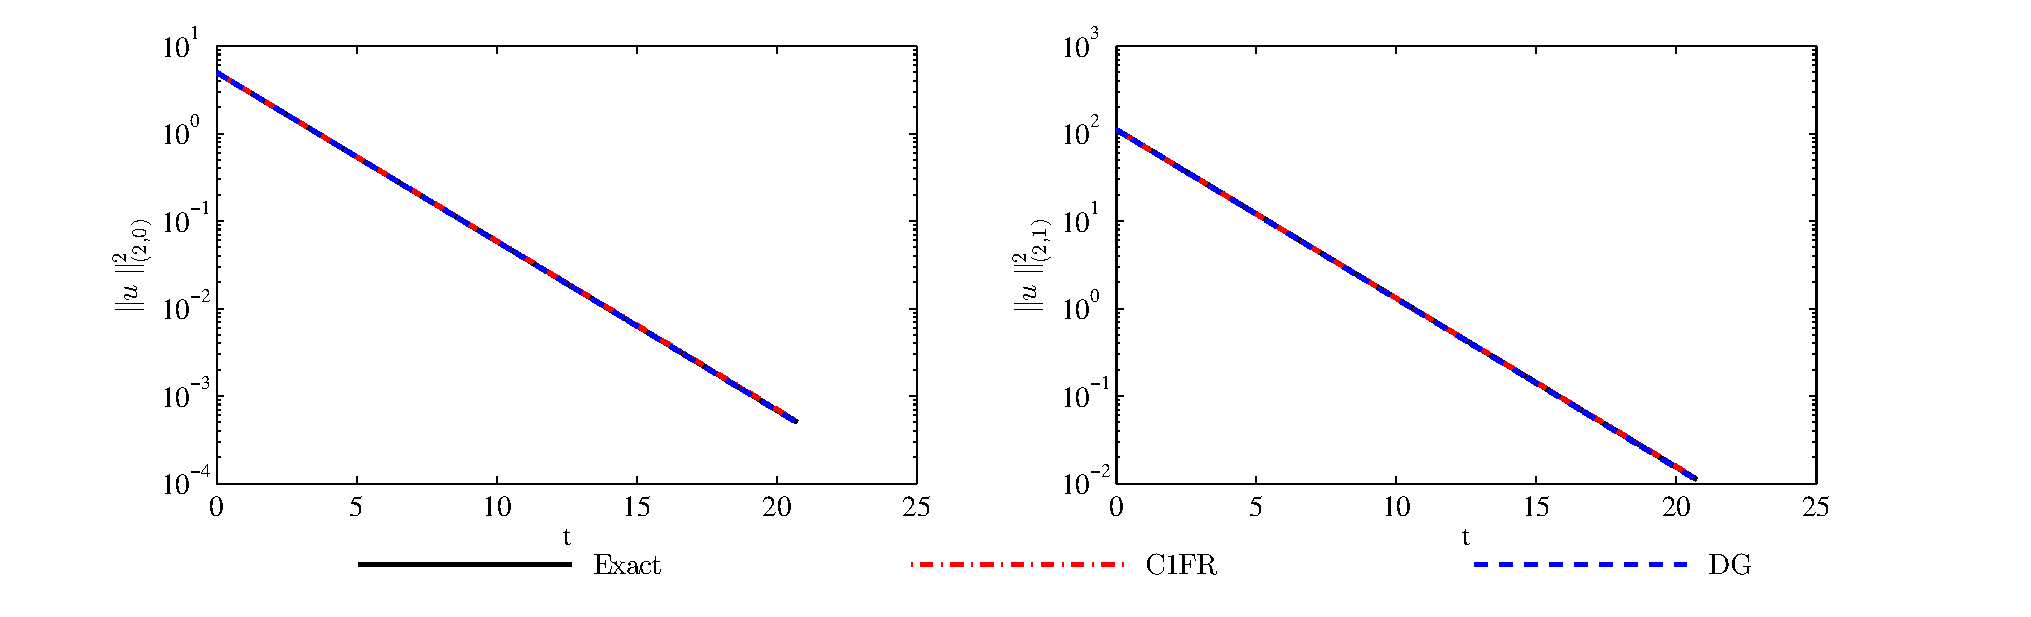
\includegraphics[width=1\textwidth,trim=\Ltrim cm 0cm \Rtrim cm 0cm]{\cmfrdir/Figures/Test_adv_diff/low_k}
\caption{Time history of norms of numerical solutions to the advection-diffusion equation and their first derivative. Initial condition is a sine wave with low wavenumber: $k = 0.25 (P+1)\pi/h$, $P = 3$, $h = 1$.}
\label{fig:low_wavenumber}
\end{figure}

\begin{figure}[h]
\centering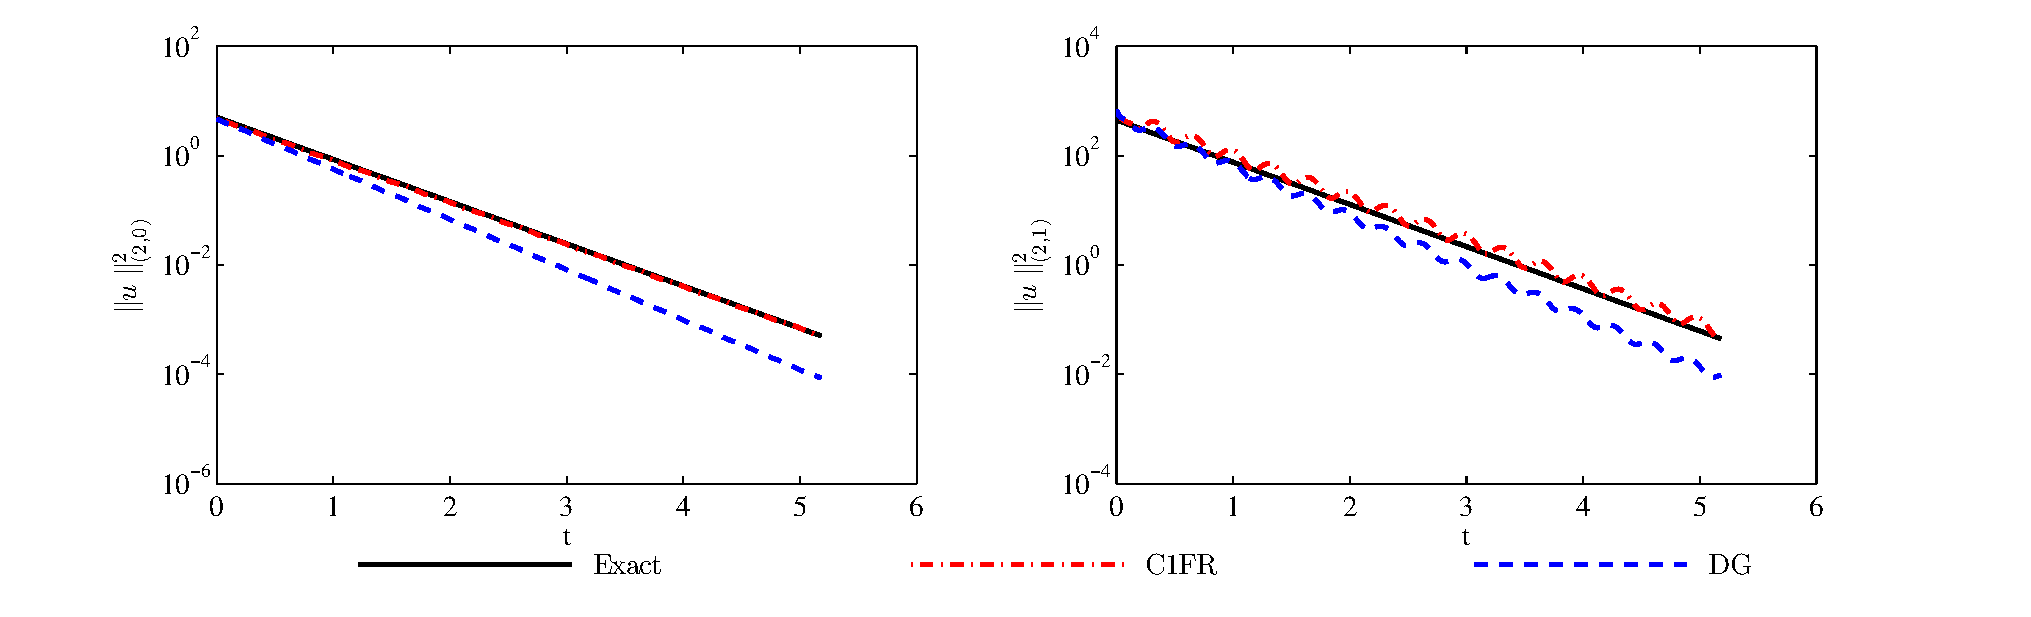
\includegraphics[width=1\textwidth,trim=\Ltrim cm 0cm \Rtrim cm 0cm]{\cmfrdir/Figures/Test_adv_diff/med_k}
\caption{Time history of norms of numerical solutions to the advection-diffusion equation and their first derivative. Initial condition is a sine wave with medium wavenumber: $k = 0.5 (P+1)\pi/h$, $P = 3$, $h = 1$.}
\label{fig:medium_wavenumber}
\end{figure}

\begin{figure}[h]
\centering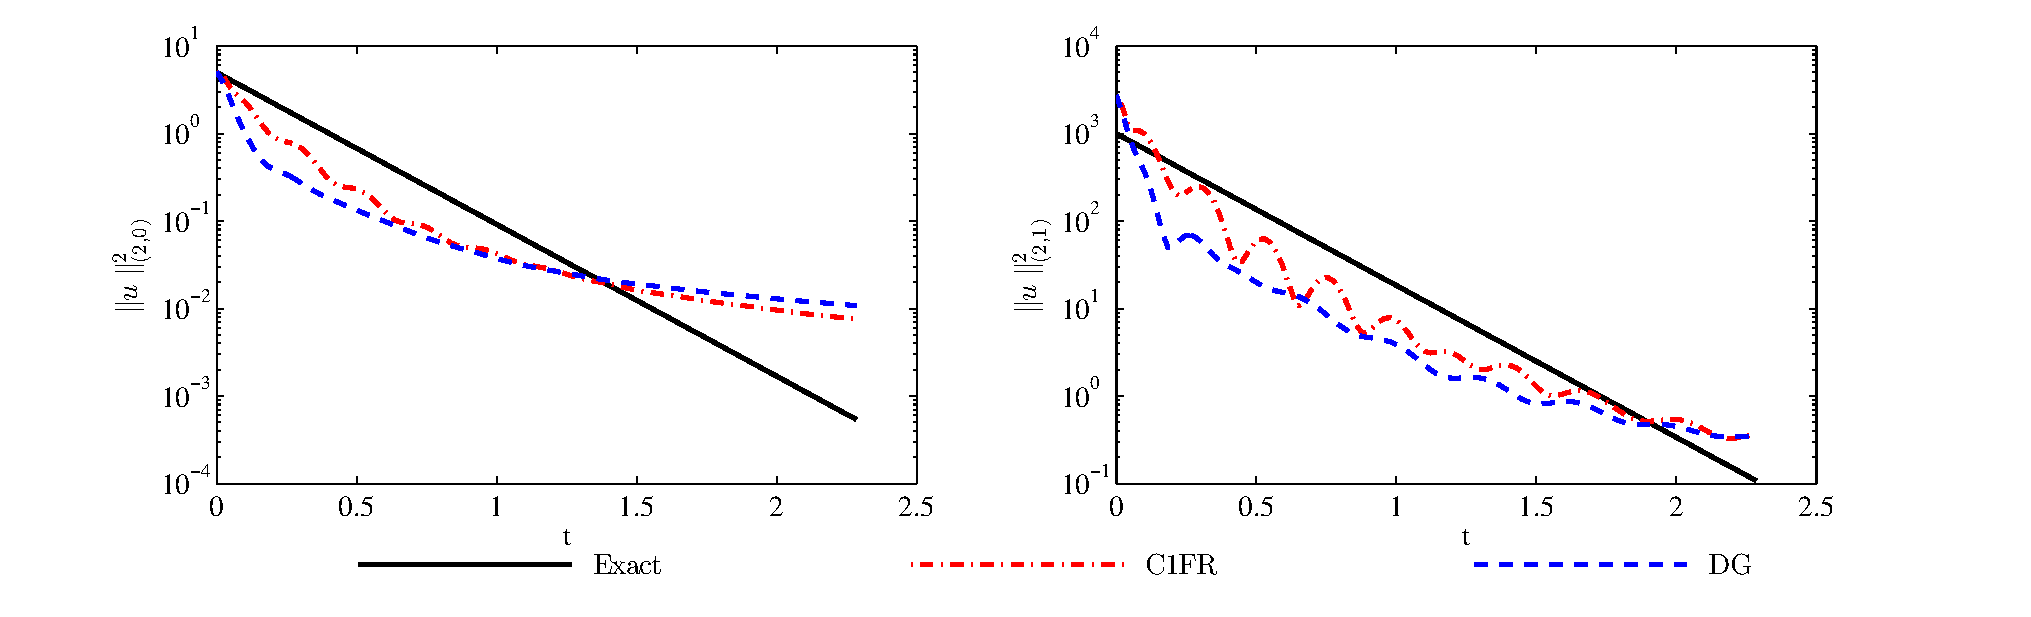
\includegraphics[width=1\textwidth,trim=\Ltrim cm 0cm \Rtrim cm 0cm]{\cmfrdir/Figures/Test_adv_diff/high_k}
\caption{Time history of norms of numerical solutions to the advection-diffusion equation and their first derivative. Initial condition is a sine wave with high wavenumber: $k = 0.75 (P+1)\pi/h$, $P = 3$, $h = 1$.}
\label{fig:high_wavenumber}
\end{figure}

%_ %_ %_ %_ %_ %_ %_ %_ %_ %_ %_ %_ %_ %_ %_ %_ %_ %
%\begin{figure}[h]
%\centering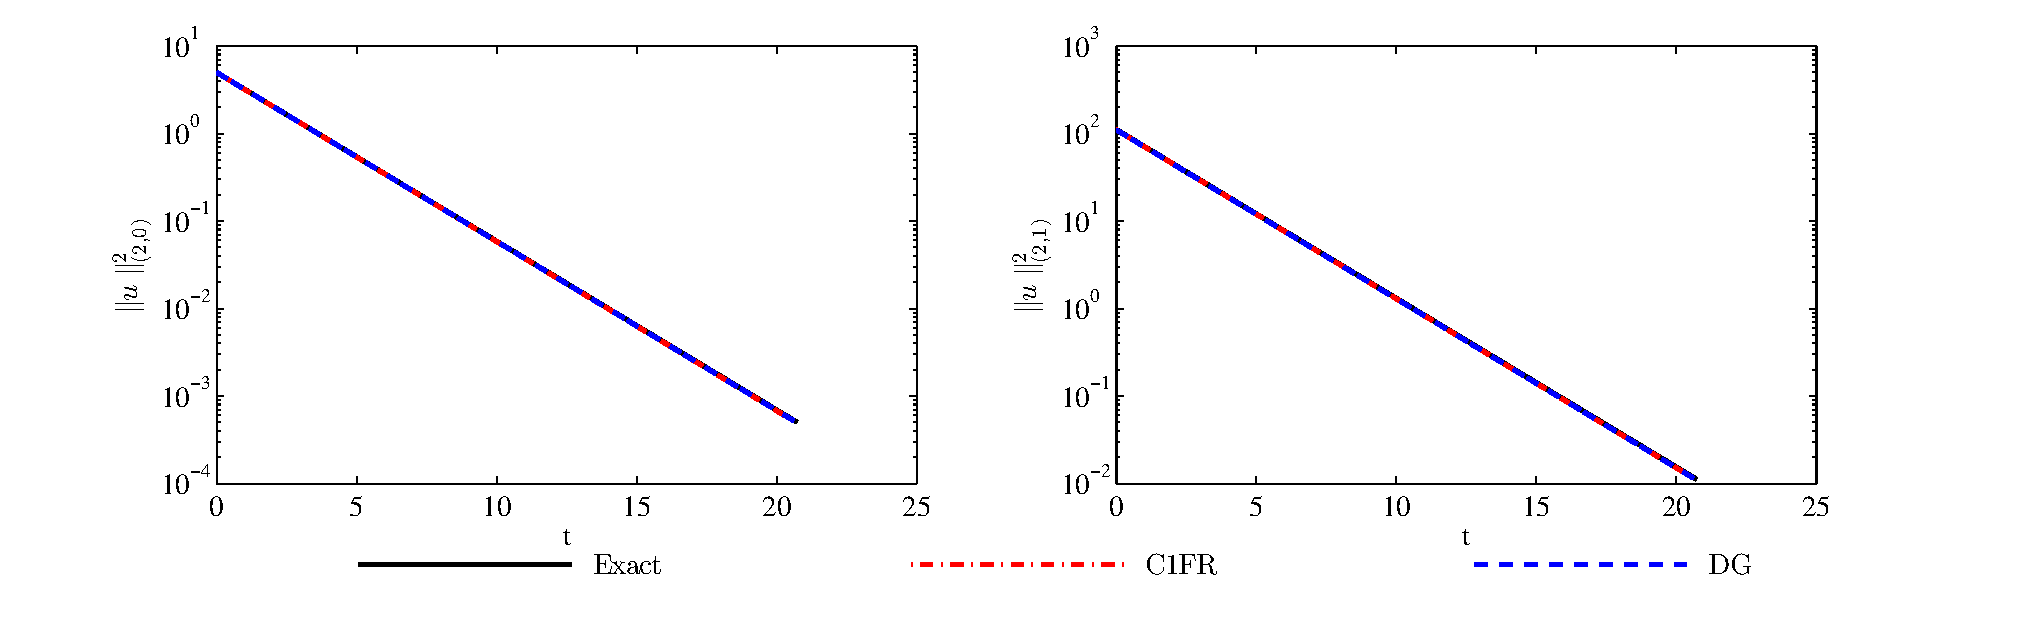
\includegraphics[width=1\textwidth,trim=\Ltrim cm 0cm \Rtrim cm 0cm]{Figures/Test_adv_diff/low_k_c_5e-3}
%\caption{Time history of norms of numerical solutions to the advection-diffusion equation and their first derivative. Initial condition is a sine wave with low wavenumber: $k = 0.25 (P+1)\pi/h$, $P = 3$, $h = 1$.}
%\label{fig:low_wavenumber2}
%\end{figure}
%
%\begin{figure}[h]
%\centering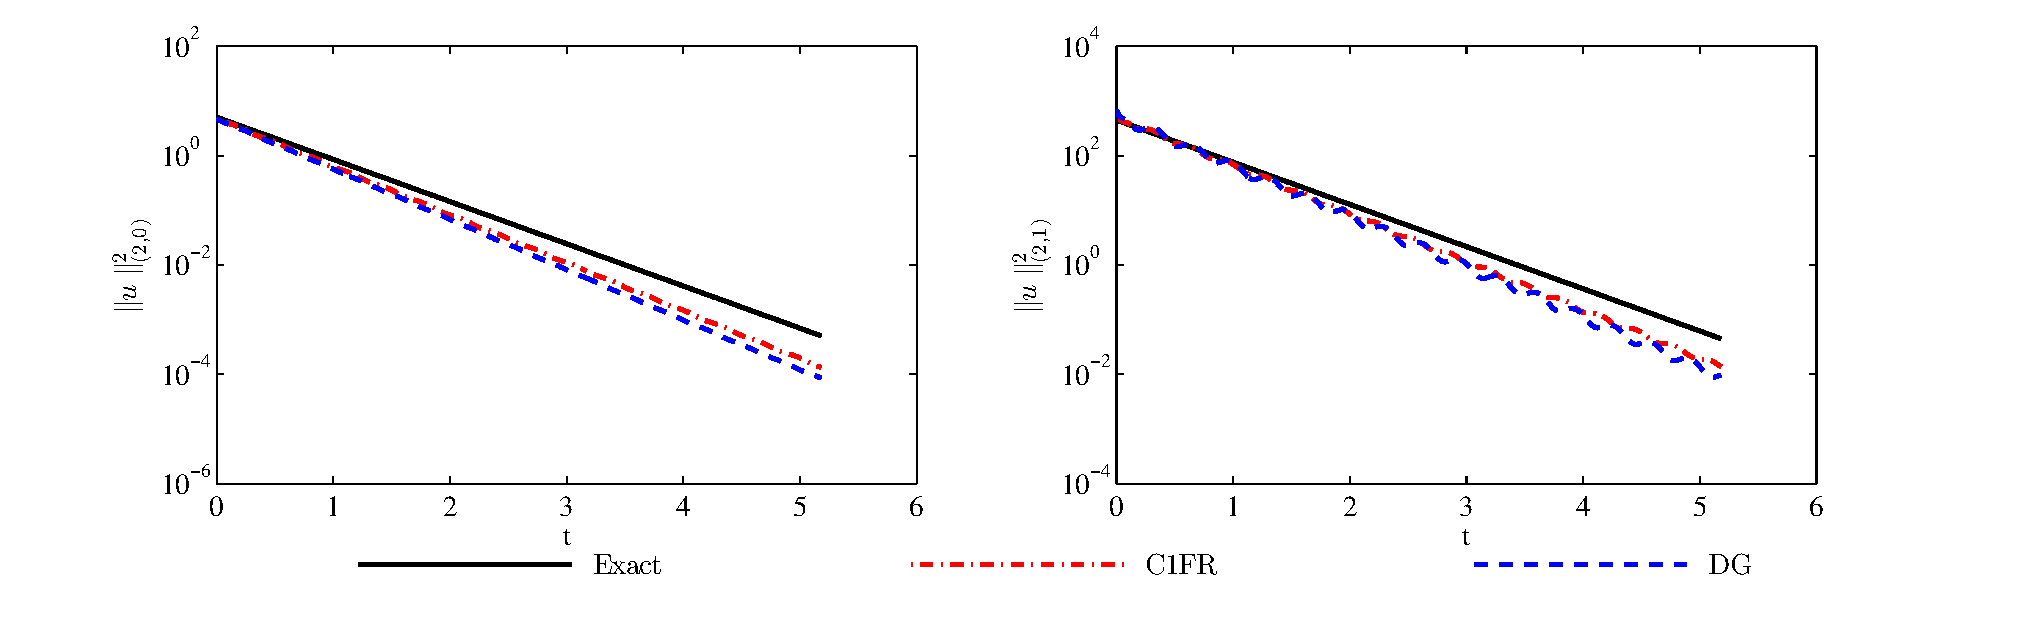
\includegraphics[width=1\textwidth,trim=\Ltrim cm 0cm \Rtrim cm 0cm]{Figures/Test_adv_diff/med_k_c_5e-3}
%\caption{Time history of norms of numerical solutions to the advection-diffusion equation and their first derivative. Initial condition is a sine wave with medium wavenumber: $k = 0.5 (P+1)\pi/h$, $P = 3$, $h = 1$.}
%\label{fig:medium_wavenumber2}
%\end{figure}
%
%\begin{figure}[h]
%\centering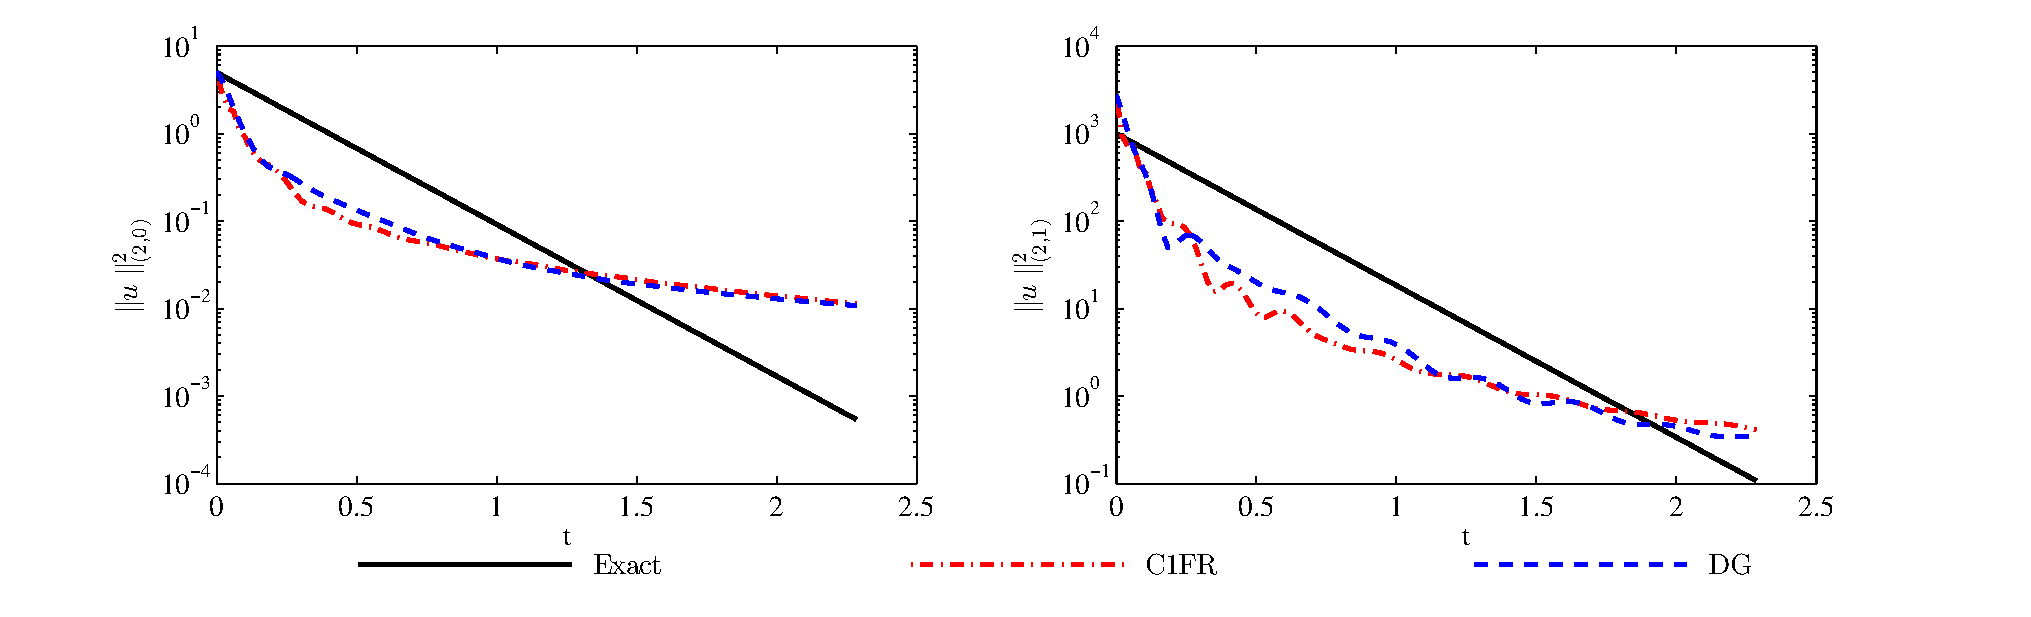
\includegraphics[width=1\textwidth,trim=\Ltrim cm 0cm \Rtrim cm 0cm]{Figures/Test_adv_diff/high_k_c_5e-3}
%\caption{Time history of norms of numerical solutions to the advection-diffusion equation and their first derivative. Initial condition is a sine wave with high wavenumber: $k = 0.75 (P+1)\pi/h$, $P = 3$, $h = 1$.}
%\label{fig:high_wavenumber2}
%\end{figure}

%_ %_ %_ %_ %_ %_ %_ %_ %_ %_ %_ %_ %_ %_ %_ %_ %_ %

%\begin{figure}
%\centering
%\subfigure[fig a]{\label{fig:high_wavenumber} 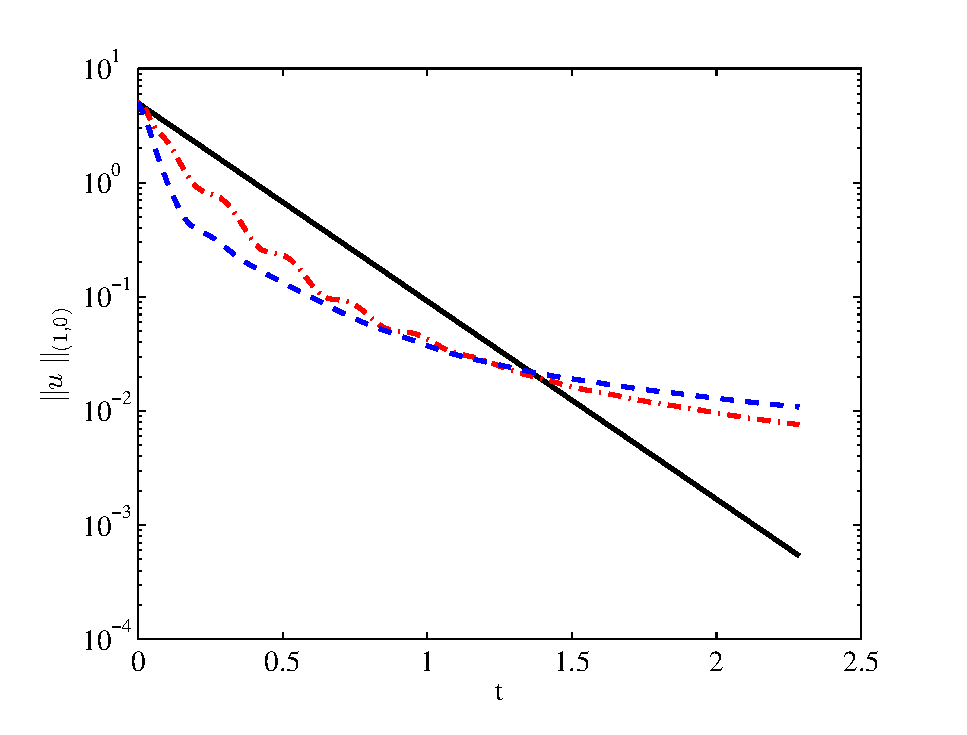
\includegraphics[width = .5\textwidth]{Figures/Test_adv_diff/eN0_high_k}
%\caption{energy history}}

%\end{subfig}
%\end{figure}

